\subsection{Аппарат частотных характеристик систем управления: амплитудно-фазовые 	характеристики; амплитудная и фазовая частотные характеристики и логарифмические 	амплитудно-фазовые частотные характеристики}

Различают два вида характеристик САУ и их звеньев: временные и частотные.

Временные характеристики (переходная, весовая) получают подавая на вход СУ эталонные сигналы: $\mathbf{1}(t), \delta(t)$. 

Частотные характеристики СУ и их звеньев получаются рассмотрением вынужденных движений системы (звена) при подаче на ее вход гармонического сигнала:
\begin{equation}
    x(t) = A \sin{\omega t},
\end{equation}
где $\omega$~--- частота.

При таком входе на выходе линейной системы в установившемся режиме (при больших $t$) будет синус той же частоты (для устойчивых систем), но с другой амплитудой $A$ и сдвигом фазы $\phi$:
\begin{equation}
    x(t) = A(\omega) \sin{(\omega t + \phi(\omega))}.
\end{equation}

Зная ПФ СУ можно вычислить амплитуду и сдвиг фазы:
\begin{equation}
    A(\omega) = |\W(j \omega)|, \quad \phi(\omega) = \arg{W(j \omega)} = \arctan{\cfrac{Im W(j \omega)}{Re W(j \omega)}}.
\end{equation}
где $j \omega = s$, т.е. в обычную ПФ вместо $s$ подставляется только мнимая ее часть.
Для кажой частсоты $\omega$ значение $W(j \omega) = P + jQ = A(\omega) e^{-j\phi(\omega)}$~--- это некторое комплексное число с амплитудой $|W(j \omega)| = \sqrt{P^2 + Q^2}$ и фазой $\arg W(j \omega) = \arctan{\cfrac{Q}{P}}$. 

ПФ $W(j \omega$~--- называется \textbf{частотной характеристикой звена}, т.к она характеризует выход системы при гармонических сигналах разной частоты. Где $P, Q$~--- вещественная и мнимая частотные характеристики.

Функции $A(\oemga), \phi(\omega)$~--- называются соответственно \textbf{амплитудной и фазовой характеристиками} (АЧХ и ФЧХ). \textit{Амплитудная характеристика}~--- это коэффициент усиления гармонического сигнала.

По форме АЧХ различают несколько основных типов звеньев:
\begin{enumerate}
    \item ФНЧ~--- пропускает низкочастотные сигналы примерно с одинаковым коэффициентом усиления, ослабляет высокочистотные шумы и помехи;
    \item ФВЧ~--- пропускает высокие, ослаблляет низкие;
    \item полосовой фильтр~--- комбинация предыдущих;
    \item полосовой режекторный фильтр~--- инвертированные предыдущий.
\end{enumerate}

\textbf{Амплитудно-фазовая частотная характеристика} (АФЧХ) — удобное представление частотного отклика линейной стационарной динамической системы в виде графика в комплексных координатах.

На комплексной плоскости $W$ (см. рисунок) комплексное число  изображается вектором ОС, длина которого равна $A(\omega)$, а аргумент это угол $\phi(\omega)$ образованный этим вектором с действительной положительной полуосью.

При изменении частоты от 0 до $\infty$ вектора ОС (точка) опишет некоторую кривую, которая называется годографом амплитудно-фазо-частотной характеристики.

\begin{figure}[h!]
    \begin{minipage}[h]{0.5\linewidth}
        \centering
        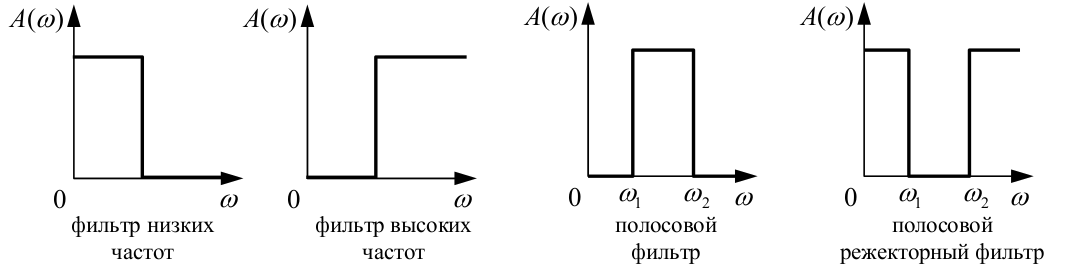
\includegraphics[width=0.8\linewidth]{images/af.png}
        \caption{Амплитудные характеристики идеальных фильтров}
        \label{fig:a_filters}    
    \end{minipage}
    \begin{minipage}[h]{0.5\linewidth}
        \centering
        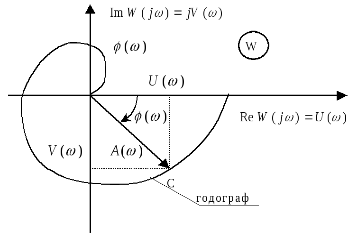
\includegraphics[width=0.5\linewidth]{images/aphf.png}
        \caption{АФЧХ}
        \label{fig:aphf}
    \end{minipage}
\end{figure}
В практике исследований систем автоматического управления широко применяются логарифмические амплитудно-частотные и фазо-частотные характеристики.

Частотные характеристики достаточно сложно строить вручную. В 60-е годы, когда раз вивалась классическая теория управления, не было мощных компьютеров, поэтому наибольшую популярность приобрели приближенные методы, с помощью которых можно было проектировать регуляторы с помощью ручных вычислений и построений. Один из таких подходов основа на использовании логарифмических частотных характеристик. 
Вместо $A(\oemga)$ было предложено использовать логарифмическую амплитудную частотных характеристику (ЛАЧХ): график, на котором по оси абсцисс откладывается десятичный лога рифм частоты $(\log\omega)$, а по оси ординат~--- величина, измеряемая в децибелах (дБ). При построении логарифмической фазовой частотной характеристики (ЛФЧХ) по оси абсцисс также откладывается логарифм частоты. Единицей отсчета на логарифмической оси частот является декада~--- диапазон, на котором частота увеличивается в 10 раз (а значение ее логарифма увеличивается на единицу). Вместе ЛАЧХ и ЛФЧХ называются логарифмической амплитудно-фазовой частотной характеристикой (ЛАФЧХ) или диаграммой Боде.

\textbf{Логарифмическая амплитудно-частотная} ЛАЧХ характеристика системы автоматического управления~--- это кривая, cоответствующая двадцати десятичным логарифмам модуля $W(j \oemga)$, построенной в десятичном логарифмическом масштабе частот~--- размерность децибел. ЛАЧФ:
\begin{equation}
    L(\omega) = 20 \log{|W(j \omega)|} = 20 \log{A(\omega)}
\end{equation}

\textbf{Логарифмическая фазо-частотная характеристика} ЛФЧХ системы автоматического управления~--- это её фазо-частотная характеристика $\phi(\omega)$, построенная в логарифмическом масштабе частот.

Ценность частотных характеристик состоит в том, что они позволяют косвенно судить о процессах, происходящих в системах автоматического управления (не решая дифференциальных уравнений, описывающих данную систему).

Для построения логарифмической амплитудно-частотной характеристики принято брать более мелкую единицу измерения, которая в 20 раз меньше одной десятичной логарифмической единицы

В ЛЧХ единица измерения ординат~--- децибел, по оси абсцисс~--- декада. Частота, для которой $A(\oemga_c) = 1$~--- называется частотой среза. Для устойчивых система значение фазына частоте среза должно быть больше $-180^o$, а годограф не должен охватывать точку $(-1, 0)$.














